\documentclass[aspectratio=169,10pt]{beamer}
\usetheme{Madrid}
\usecolortheme{default}
\usefonttheme{professionalfonts}
\setbeamertemplate{navigation symbols}{}
\setbeamertemplate{footline}[frame number]
\usepackage[T1]{fontenc}
\usepackage[utf8]{inputenc}
\usepackage{lmodern}
\usepackage{xcolor}
\usepackage{tikz}
\usetikzlibrary{positioning,arrows.meta}
\usepackage{listings}
\usepackage{hyperref}
\definecolor{LabBlue}{RGB}{25,76,153}
\definecolor{LabGreen}{RGB}{0,101,87}
\setbeamercolor{structure}{fg=LabBlue}
\lstset{basicstyle=\ttfamily\scriptsize,breaklines=true,columns=fullflexible,showstringspaces=false,frame=single,keywordstyle=\color{LabBlue}}

\title[L03 - Agent Engineering]{L03: Framework orchestration: LangGraph and SDK alternatives}
\subtitle{Week 03 | M02 | Scaffold - NOT IMPLEMENTED}
\author{AI Agent Engineering Curriculum}
\date{November 2026 | 1.0}
\begin{document}
\begin{frame}\titlepage\end{frame}

\begin{frame}{Laboratory learning contract}
\small
\begin{itemize}
\item Module M02, LO03, syllabus Section 13 p27.
\item Implement equivalent routing using a graph and the handcrafted runner.
\item 4 hours implementation; 1.5 hours verification; total weekly effort 10 hours.
\item Submit typed code, diagram, tests, security note and independently validated evidence.
\end{itemize}

\end{frame}

\begin{frame}{Prerequisites and current status}
\small
\begin{itemize}
\item Source repository status: Scaffold - NOT IMPLEMENTED.
\item Prerequisite: prior labs through L02 and their safety gates.
\item Start offline with FakeModel and mock provider; no paid API or cloud access is required.
\item A scaffold or evidence placeholder never proves implementation.
\end{itemize}

\end{frame}

\begin{frame}{Engineering problem and target}
\small
\begin{itemize}
\item Implement equivalent routing using a graph and the handcrafted runner.
\item Exit criteria: Graph reproducible; trade-off evaluation has ≥6 criteria and ≥3 technologies; a clean offline checkout must reproduce the result with a fixed test seed, and evidence.json must record commit SHA, run ID, versions, check status, and r...
\item The success predicate must be independently testable and source-backed.
\end{itemize}

\end{frame}

\begin{frame}{Core concepts and technical vocabulary}
\small
\begin{itemize}
\item Typed graph with guarded routing, framework parity tests and ADR
\item Input contracts and typed outputs define the trusted execution boundary.
\item A model answer is an observation, not an authorization or verified completion.
\end{itemize}

\end{frame}

\begin{frame}{Architecture patterns and trade-offs}
\small
\begin{itemize}
\item Typed graph with guarded routing, framework parity tests and ADR
\item Compare extensibility, deterministic behavior, isolation, cost and evidence fidelity.
\item Keep business authorization outside framework-specific orchestration.
\item Document selected design and rejected alternatives in source-controlled decisions.
\end{itemize}

\end{frame}

\begin{frame}{Architecture and data flow}
\small
\centering
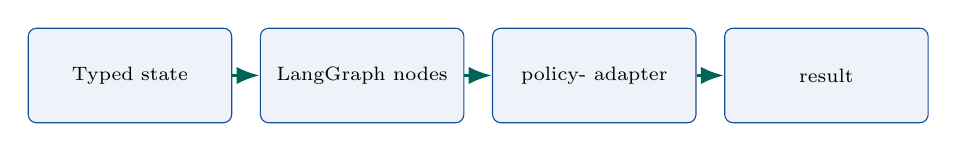
\begin{tikzpicture}[node distance=0.35cm,>=Latex,stagebox/.style={draw=LabBlue,fill=LabBlue!7,rounded corners=3pt,minimum height=1.2cm,minimum width=2.55cm,text width=2.35cm,align=center,font=\scriptsize}]
\node[stagebox] (n0) {Typed state};
\node[stagebox,right=of n0] (n1) {LangGraph nodes};
\node[stagebox,right=of n1] (n2) {policy- adapter};
\node[stagebox,right=of n2] (n3) {result};
\draw[->,very thick,LabGreen] (n0) -- (n1);
\draw[->,very thick,LabGreen] (n1) -- (n2);
\draw[->,very thick,LabGreen] (n2) -- (n3);
\end{tikzpicture}
\vspace{0.6cm}
\begin{block}{Trust boundary}
Model proposals do not grant access. The harness validates, policy adjudicates, and resources enforce permission.
\end{block}
\end{frame}

\begin{frame}{Responsibility boundaries}
\small
\begin{itemize}
\item Model: untrusted proposal and generated explanation.
\item Framework: optional workflow nodes and state orchestration.
\item Harness: tool allowlisting, schemas, budgets, dispatch, trace and recovery.
\item MCP: versioned capability exchange; tool listing is not permission.
\item Governance and resource: independent access policy, identity and reviews.
\end{itemize}

\end{frame}

\begin{frame}{Mathematical invariant}
\small
\begin{center}\Large $G=(V,E),\quad\delta:V\times S\rightarrow V$\end{center}
\begin{itemize}
\item Define each measured predicate or bound explicitly.
\item Construct a negative fixture violating at least one precondition.
\item Check the actual side effect, denial, or metric rather than model rhetoric.
\end{itemize}

\end{frame}

\begin{frame}{Technology prerequisites and contracts}
\small
\begin{itemize}
\item Python 3, pytest, typed model stub, fixtures and Git; add only the week-specific dependencies (MCP SDK in L06--07, OPA in L10, OpenTelemetry in L13, Docker in L14); pin each one in the lockfile.
\item Define typed interfaces and schema version before implementation.
\item Pin dependency revisions; run synthetic fixtures before adding external SDKs.
\item Require explicit caller identity and repository scope when relevant.
\end{itemize}

\end{frame}

\begin{frame}{System component ownership}
\small
\begin{itemize}
\item Typed graph with guarded routing, framework parity tests and ADR
\item Model/worker proposes and observes, never grants new privileges.
\item Policy enforcement checks tool, actor, scope and budget before dispatch.
\item Verifier validates the evidence against documented success predicates.
\end{itemize}

\end{frame}

\begin{frame}{Implementation I: contracts}
\small
\begin{itemize}
\item Define typed request/result/error contracts;
\item implement Build analysis$\rightarrow$retrieve$\rightarrow$verify$\rightarrow$report nodes with a typed state; maintain same external contracts as W2;
\item Write a failing security-negative test before external integration.
\end{itemize}

\end{frame}

\begin{frame}{Implementation II: guarded execution}
\small
\begin{itemize}
\item add fixtures and logging with immutable run IDs;
\item write security-first negative tests before any live integration;
\item Preserve run ID, source SHA, sanitized event stream and terminal status.
\end{itemize}

\end{frame}

\begin{frame}{Implementation III: evidence and recovery}
\small
\begin{itemize}
\item commit a design/decision diagram;
\item capture verification evidence and compare results with the week's stated rubric.
\item Capture honest evidence: versions, tester, timestamp and result.
\item Mark features planned until actual tests pass.
\end{itemize}

\end{frame}

\begin{frame}[fragile]{Code walkthrough}
\small
\begin{block}{Synthetic teaching pseudocode - not implemented}\end{block}
\begin{lstlisting}[language=Python]
def verify_node(state):
    if not state.get("evidence_ids"):
        return {"status": "blocked"}
    return {"status": "verified"}
\end{lstlisting}

\end{frame}

\begin{frame}{Hands-on laboratory sequence}
\small
\begin{itemize}
\item Read labs/L03/README.md, main.py, diagram.mmd and security.md.
\item Baseline status: Scaffold - NOT IMPLEMENTED.
\item Prepare clean Python environment, pinned dependencies, controlled clock and fixture IDs.
\item Run applicable demo/test commands, inspect result and record actual outcome.
\end{itemize}

\end{frame}

\begin{frame}{Positive path and verification}
\small
\begin{itemize}
\item correct branch and report match the reference implementation.
\item Arrange an authorized input with deterministic mock resources.
\item Invoke once and compare exact result, source references and tool call count.
\item Log independent assertions and reviewer evidence.
\end{itemize}

\end{frame}

\begin{frame}{Negative and adversarial verification}
\small
\begin{itemize}
\item unauthorized graph branch and malformed state rejected.
\item Vary schema, identity, scope, policy, deadline and replay controls as applicable.
\item Observe real dispatcher/API side effects in a mock environment.
\item All mandatory authorization-negative cases are hard blockers.
\end{itemize}

\end{frame}

\begin{frame}{Security and least privilege}
\small
\begin{itemize}
\item Enforce authorization in application-owned adapters not only model instructions.
\item Treat prompts, retrieved files, issues and MCP tool responses as untrusted.
\item Keep shell, network and all real GitHub write/dismissal routes disabled by default.
\item Record explicit policy denial and redact evidence.
\end{itemize}

\end{frame}

\begin{frame}{Fault handling and recovery}
\small
\begin{itemize}
\item If state mutates unexpectedly, inspect reducer merges and immutable fixture snapshots.
\item Distinguish blocked, failed, cancelled, needs\_approval and budget\_exhausted.
\item Use idempotency or checkpoint reconciliation before any retry.
\item Do not silently recover an unauthorized operation.
\end{itemize}

\end{frame}

\begin{frame}{Reproducibility and evidence}
\small
\begin{itemize}
\item Evidence.json records source SHA, run ID, timestamp, tool versions, tester and status.
\item Include diagram, security note and positive/negative test report.
\item Pin Python and protocol revisions, fix fixture seeds, and run offline.
\item The recorded result must not be not\_started or unverified.
\end{itemize}

\end{frame}

\begin{frame}{Acceptance criteria}
\small
\begin{itemize}
\item Graph reproducible
\item trade-off evaluation has ≥6 criteria and ≥3 technologies
\item a clean offline checkout must reproduce the result with a fixed test seed, and evidence.json must record commit SHA, run ID, versions, check status, and reviewer/tester.
\item Reject a lab if any required authorization-negative case fails.
\item Independently verify every negative authorization gate.
\end{itemize}

\end{frame}

\begin{frame}{Assessment rubric}
\small
\begin{itemize}
\item correct architecture and contracts 20; implementation and type correctness 25; positive/negative tests 30; security and error handling 15; reproducibility and documentation 10.
\item source, fixture data, diagram, tests, evidence log and a one-page engineering summary. Advanced extension: port the contract to TypeScript/Java or run an independently authorized clo...
\item A reviewer must reproduce the recorded commands and outcomes.
\end{itemize}

\end{frame}

\begin{frame}{Instructor review questions}
\small
\begin{itemize}
\item Which security component owns authority in L03?
\item Can 'correct branch and report match the reference implementation.' pass despite unsafe authorization?
\item How would you reproduce 'unauthorized graph branch and malformed state rejected.'?
\item Which exact source revision and evidence IDs prove completion?
\end{itemize}

\end{frame}

\begin{frame}{Optional advanced extension}
\small
\begin{itemize}
\item Advanced features must be pinned, independently tested and explicitly scoped.
\item No advanced work waives a failed safety or reproducibility gate.
\end{itemize}

\end{frame}

\begin{frame}{References and provenance}
\small
\begin{itemize}
\item Syllabus Section 7 Week 3 and Section 13 p27.
\item Read labs/L03/README.md, security.md, diagram.mmd and source tests.
\item Pinned source commit: 3b62f5ad71796489c5f6813ad9e53e41a54211cd.
\item Check official, current protocol/library references against pinned versions.
\end{itemize}

\end{frame}

\begin{frame}{Completion and next steps}
\small
\begin{itemize}
\item Objective: Graph reproducible; trade-off evaluation has ≥6 criteria and ≥3 technologies; a clean offline checkout must reproduce the result with a fixed test seed, and evidence.j...
\item Commit code, design, tests and true run evidence after verification.
\item Demonstrate both successful behavior and a blocked adversarial path.
\item Proceed to L04 only after passing this gate.
\end{itemize}

\end{frame}

\end{document}
